\subsection{Molten Salt Reactors}

\begin{frame}
\frametitle{Potential Generation IV reactor systems \cite{abram_generation-iv_2008}}
\begin{figure}[t]
	\vspace*{-0.1in}
	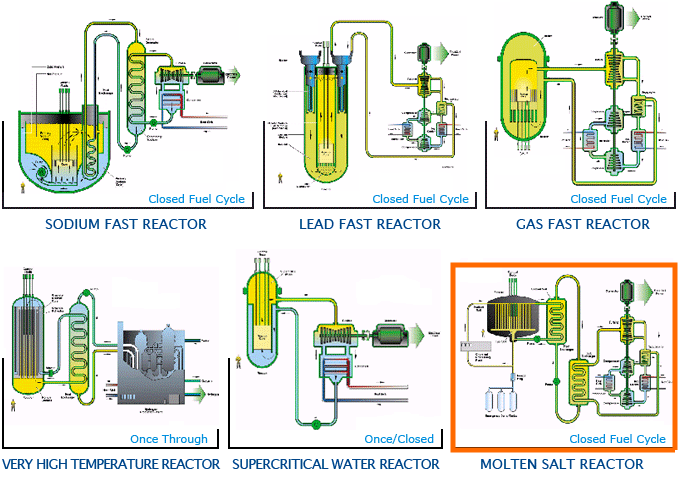
\includegraphics[height=0.7\textwidth]{./images/6_types.png}
	\caption{\gls{MSR} design}
\end{figure}            
\end{frame}


\begin{frame}
\frametitle{MSR (Molten Salt Reactor) types}
\begin{overlayarea}{\linewidth}{20\baselineskip}
\begin{block}{Stationary Fuel}<1-4>
	\begin{enumerate}
		\item Graphite block with TRISO fuel, clean salt works as 
		coolant (Fluoride-Salt-Cooled High-Temperature 
		Reactor (FHR))
		\item Plate Fuel: hexagonal fuel assembly is similar in shape to a typical sodium-cooled reactor
		\item Fuel Inside Radial Moderator (FIRM)
		\item Liquid fuel salt inside fuel rods cooled by clean salt 
		(Moltex Stable Salt Reactor)
	\end{enumerate}
\end{block}

\begin{block}{Mobile Fuel}<2-4>
	\begin{enumerate}
		\item<2-4> Mobile solid fuel elements (pebbles) cooled by 
		clean salt (PB-FHR)
		\item<3-4> Non-circulating liquid fuel salt (TerraPower \gls{MCFR}) 
		\item<4> \textbf{Circulating liquid fuel salt} which also works 
		as coolant (\gls{MSBR})
	\end{enumerate}
\end{block}
\end{overlayarea}
\end{frame}


\begin{frame}
\frametitle{Stationary and Mobile Solid fuel}
\vspace*{-0.1in}
\begin{figure}[t]
	\hspace*{-0.35in}
	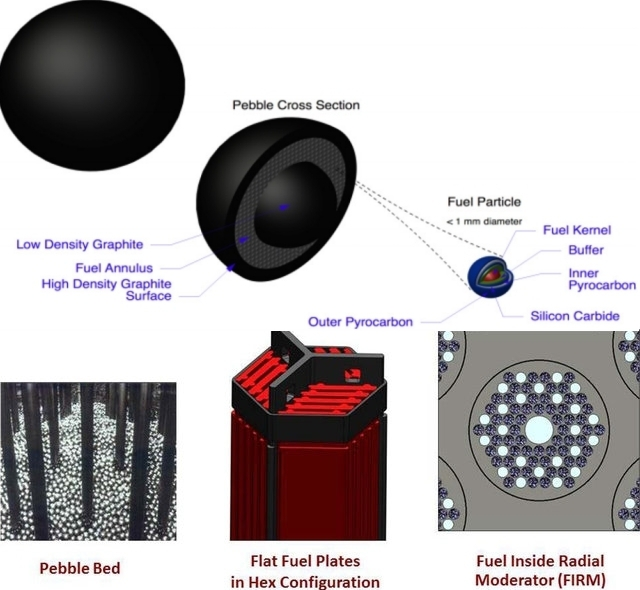
\includegraphics[height=0.63\textwidth]{./images/solid_fuel.jpg}
	\caption{TRISO fuel particle (top) and FHR fuel designs (bottom). Source \cite{forsberg_basis_2016}.} 
\end{figure}   
\end{frame}

\begin{frame}
\frametitle{Mobile, Non-Circulating, Liquid Fuel}
\begin{figure}[t]
\vspace*{-0.1in}
\hspace*{-0.35in}
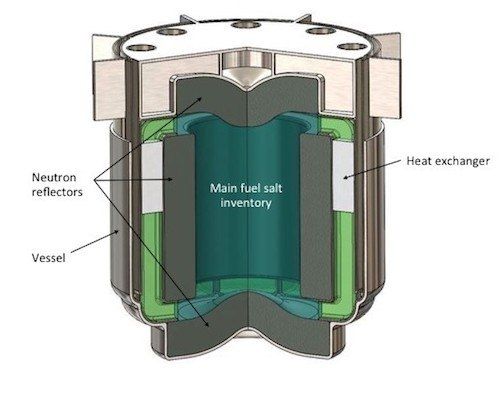
\includegraphics[height=0.6\textwidth]{./images/mcfr-crossection.jpg}
\caption{The TerraPower MCFR is an example of reactor design with \textbf{liquid, mobile, non-circulating} chloride salt fuel. Source \cite{doene_southern_2018}.}
\end{figure}   

\end{frame}


\begin{frame} % Add another slide with red rectangular around reprocessing system
\frametitle{Mobile, Circulating, Liquid Fuel}
\begin{figure}[t]
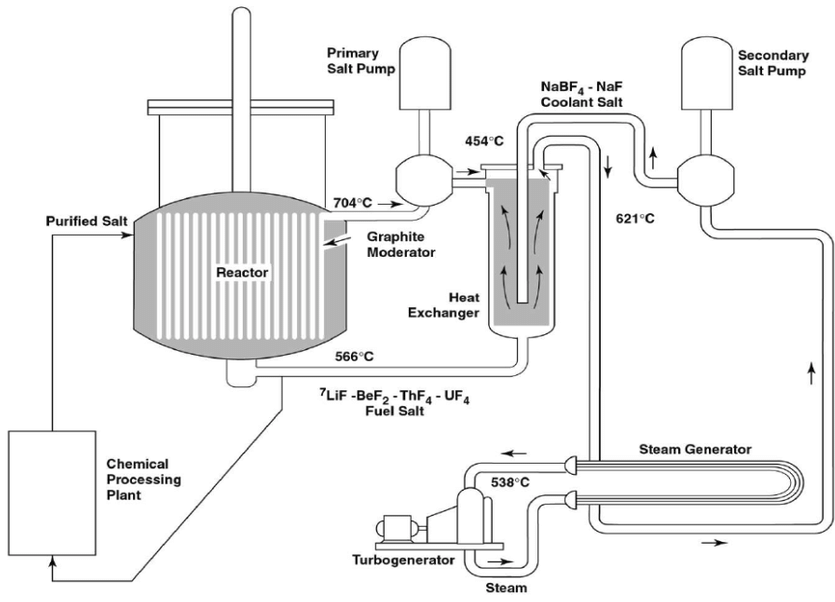
\includegraphics[height=0.58\textwidth]{./images/msbr_scheme.png}
\caption{The \gls{MSBR} is an example of reactor design with \textbf{liquid, mobile, circulating} fluoride salt fuel \cite{rosenthal_molten-salt_1970}.}
\end{figure}   

\end{frame}

\begin{frame}
\frametitle{Why Molten Salt Reactors with circulating fuel?}
\begin{block}{Liquid-fueled \gls{MSR} designs have following \textbf{potential} advantages:}
	\begin{enumerate}
		\itemsep1em
		\item High coolant temperature (600-750$^{\circ}$C) 
		$\Rightarrow$ potentially high thermal efficiency, process 
		heat for chemical industry
		\item Fuel diversity ($^{235}$U, $^{233}$U, Thorium, U/Pu)
		\item Strong negative temperature feedback of liquid fuel
		\item Passive safety $\Rightarrow$ fuel drains into tanks 
		in emergency
		\item High fuel utilization $\Rightarrow$ less nuclear 
		waste generated
		\item<2> \textbf{On-line (continuous) fuel reprocessing and refueling}
	\end{enumerate}
\end{block}

\end{frame}


\subsection{Background}


\begin{frame}
\frametitle{On-line fuel processing and online refueling pros and cons}
\begin{block}{Advantages}
	\begin{enumerate}
		\item Improved neutrons economy
		\item Better fuel utilization
		\item Smaller excess reactivity
		\item Ability to maintain criticality without shutdown
	\end{enumerate}
\end{block}

\begin{block}{Disadvantages}
	\begin{enumerate}
		\item Chemical separation is challenging
		\item Fuel salt balance in a primary loop complicates operation
		\item \textbf{Hard to model using most contemporary burnup software}
	\end{enumerate}
\end{block}

\end{frame}


\begin{frame}
\frametitle{Fuel salt burnup and reprocessing}
\vspace*{-0.05in}
\begin{enumerate}
	\item Gaseous fission products escape (50\% removal efficiency) from the fuel salt
	\item Noble metals (Mo, Tc) plate out on surfaces
	\item Rare earth metals should be removed by chemical processing
	\item Most of burnup codes cannot treat fuel movement
\end{enumerate}

\begin{figure}[t]
	\hspace*{-0.2in}
	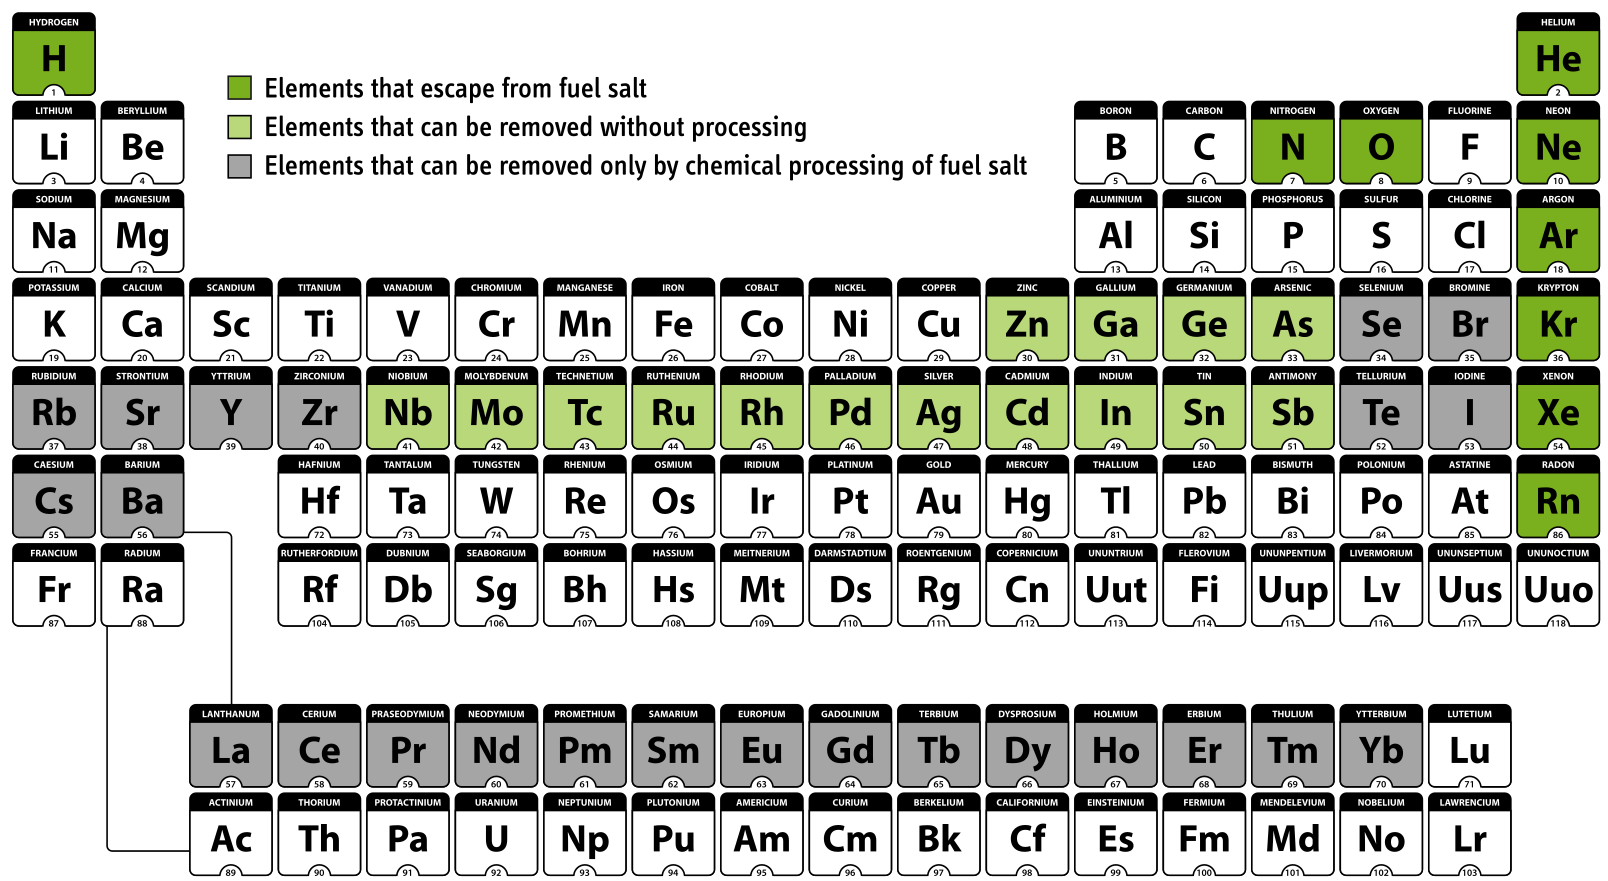
\includegraphics[height=0.48\textwidth]{../figures/periodic_map.png}
	\vspace*{-0.05in}
	\caption{Processing options for MSR fuels (figure reproduced from Ahmed et al. \cite{ahmad_neutronics_2015}).}
\end{figure}               
\end{frame}


\begin{frame}
\frametitle{On-line fuel salt reprocessing system functions}
\begin{block}{Removal poisonous fission products from the salt}
	\begin{itemize}
		\item Enhance noble gases escape (e.g., by ejecting helium or using centrifugal gas separator)
		\item Improve noble metals removal (e.g., nickel filter with large metal surface)
		\item Remove rare earths using difference in chemical potentials
		\item Ideally, 100\% of target element but realistically - 30-90\%
		\item Some rare metals (Rh,Pd) might be economically recovered from waste stream %Rh - $5000, Pd - $1500, Pl - $900, Ir - $1480
	\end{itemize}
\end{block}

\begin{block}{Feed (inject) fresh fuel to the salt}
	\begin{itemize}
		\item Inject fissile material ($^{233}$U, $^{235}$U, $^{239}$Pu)
		\item Inject fertile material ($^{232}$Th, $^{238}$U)
		\item Maintain fuel salt inventory in the primary loop
		\item Maintain the reactor critical (ideally, $k_{eff}=1.0$)
	\end{itemize}
\end{block}

\end{frame}


\begin{frame}
\frametitle{Fuel salt reprocessing approaches}

Fuel salt is circulated throughout fuel reprocessing system:
\\
\begin{enumerate}
	\itemsep2em
	\item Continuously:
	\begin{itemize}
		\item removal and feed terms are added to the Bateman equation
		\item relatively coarse burnup timesteps needed
	\end{itemize}
	\item At specific intervals (batch-wise): 
	\begin{itemize}
		\item the
burn-up simulation stops at a given time and restarts with a new
liquid fuel composition (after removal of discarded materials and
		addition of fissile/fertile materials)
		\item very fine burnup timesteps needed
	\end{itemize}
\end{enumerate}


\end{frame}


\begin{frame}
\frametitle{Continuous vs batch-wise fuel processing  and refueling (1/3)}
\vspace{-7mm}
\begin{block}{Classic Bateman equation}
	%Core material is circulated to or from the core at specific intervals:
	\begin{align}
	\frac{dN_i}{dt} &= \sum_{m=1}^{M}l_{im}\lambda_mN_m + 
	\phi\sum_{m=1}^{M}f_{im}\sigma_mN_m - (\lambda_i + \phi\sigma_i)N_i + F_i\Big|{i\in [1,M]} \nonumber\\
	N_i &= \mbox{atom density of nuclide i} \nonumber \\
	M &= \mbox{number of nuclides} \nonumber \\
	l_{im} &= \mbox{fraction of decays of nuclide m that result in formation of 
		nuclide i}\nonumber \\
	\lambda_i &= \mbox{radioactive decay constant of nuclide i} \nonumber \\
	\phi &= \mbox{neutron flux, averaged over position and energy} \nonumber \\
	f_{im} &= \mbox{fraction of neutron absorption by nuclide m leading to the 
		formation of nuclide i} \nonumber \\
	\sigma_m &= \mbox{average neutron absorption cross section of nuclide m} 
	\nonumber \\
	F_i &= \mbox{production rate of nuclide i directly from fission}\nonumber
	\end{align}
\end{block}
\end{frame}


\begin{frame}
\frametitle{Continuous vs batch-wise fuel processing  and refueling (2/3)}
\begin{block}{Bateman equation with continuous removals and feed}
	\hspace{-0.4in}
	\begin{align}
	\frac{dN_i}{dt} &= \sum_{m=1}^{M}l_{im}\lambda_mN_m + 
	\phi\sum_{m=1}^{M}f_{im}\sigma_mN_m - (\lambda_i + \phi\sigma_i + \textcolor{red}{r_i - 
	f_i})N_i + F_i\Big|{i\in [1,M]} \nonumber \\
	N_i &= \mbox{atom density of nuclide i} \nonumber \\
	M &= \mbox{number of nuclides} \nonumber \\
	l_{im} &= \mbox{fraction of decays of nuclide m that result in formation of 
		nuclide i}\nonumber \\
	\lambda_i &= \mbox{radioactive decay constant of nuclide i} \nonumber \\
	\phi &= \mbox{neutron flux, averaged over position and energy} \nonumber \\
	f_{im} &= \mbox{fraction of neutron absorption by nuclide m leading to the 
		formation of nuclide i} \nonumber \\
	\sigma_m &= \mbox{average neutron absorption cross section of nuclide m} 
	\nonumber \\
	\textcolor{red}{r_i} & \mkern4mu \textcolor{red}{=} \mbox{\space \textcolor{red}{continuous removal rate of nuclide i from the system}} \nonumber \\
	\textcolor{red}{f_i} & \mkern4mu  \textcolor{red}{=} \mbox{\space \textcolor{red}{continuous feed rate of nuclide i}} \nonumber \\
	F_i &= \mbox{production rate of nuclide i directly from fission}\nonumber
	\end{align}
\end{block}

\end{frame}

\begin{frame}
\frametitle{Continuous vs batch-wise fuel processing and refueling (3/3)}
	\begin{block}{Batch-wise approach}
		Core material is circulated to or from the core at specific intervals		
	\end{block}
           \begin{figure}[t]
	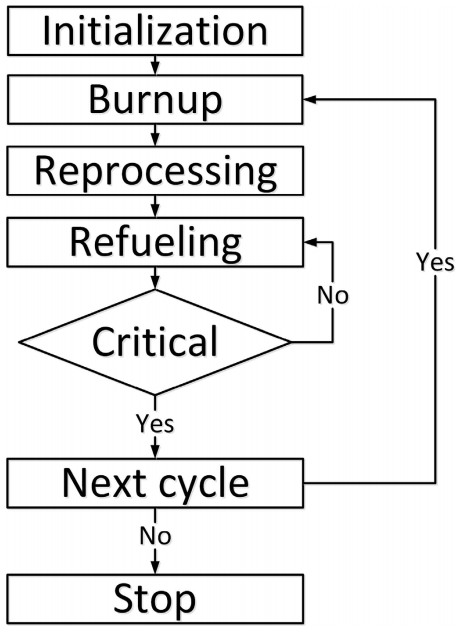
\includegraphics[height=0.45\textwidth]{./images/batch-wise.png}
	\caption{Typical flowchart for batch-wise reprocessing and refueling (figure reproduced from Li et al.\cite{li_optimization_2018}).}
			\end{figure}               
\end{frame}

\begin{frame}
\frametitle{Published work in online reprocessing and modeling}

  \begin{textblock*}{12.5cm}(0.1cm,1.9cm) % {block width} (coords)
	\begin{table}[t]
	\fontsize{6}{9}\selectfont
	\caption{Tools and methods for liquid-fueled \glspl{MSR} fuel salt depletion 
		analysis.}
	\begin{tabularx}{\textwidth}{X X X X p{3cm}} 
		\hline 
		&Nuttin \emph{et al.}, 2005 \cite{nuttin_potential_2005}& Aufiero \emph{et al.}, 
		2013 \cite{aufiero_extended_2013} & Betzler \emph{et al.}, 2018 
		\cite{betzler_fuel_2018}&Proposed work \\ 
		\hline
		Neutron transport software & \gls{MCNP} & Serpent 2 & SCALE6.2 & Serpent 2 \\ 
		Neutron transport method & \multicolumn{2}{c}{Monte Carlo continuous energy} & 
		Deterministic discrete ordinates & Monte Carlo continuous energy \\
		Burnup software & REM & Serpent 2 & ORIGEN-S & Serpent 2 \\ 
		Geometry model & unit cell & full-core 3D & unit cell & full-core 3D\\ [12pt]
		Removal/feed  & continuous &continuous & batch-wise & batch-wise\\ 
		Separation efficiency &\multicolumn{3}{c}{fixed, must be defined by user 
			before simulation} & variable of many parameters \\
		Fuel reprocessing plant & \multicolumn{3}{c}{single component, ``black'' box 
			model} & realistic multi-component model \\
		Reactivity control & \multicolumn{2}{c}{continuous adjustment of fissile 
			material injection} & batch injection of fissile material & periodical 
		adjustment of geometry and fissile material injection\\
		\hline
	\end{tabularx}
	\label{tab:msr_codes}
\end{table}
\end{textblock*}

\end{frame}


\begin{frame}
\frametitle{Past published work shortcomings}
\vspace{-0.2in}
\begin{block}{Static ``black'' box assumptions}
	\begin{equation*}
	{\tiny  
		\setlength{\abovedisplayskip}{6pt}
		\setlength{\belowdisplayskip}{\abovedisplayskip}
		\setlength{\abovedisplayshortskip}{0pt}
		\setlength{\belowdisplayshortskip}{3pt}
	\begin{aligned}
	\begin{bmatrix}
	N^{in}_{0} \\ \vdots \\ N^{in}_{e} \\ \vdots \\ N^{in}_{E} \\
	\end{bmatrix} 
	\times
	\begin{bmatrix}
	\epsilon_{0} \\ \vdots \\ \epsilon_{e} \\ \vdots \\ \epsilon_{E} \\
	\end{bmatrix} =
	\begin{bmatrix}
	N^{out}_{0}\\ \vdots \\ N^{out}_{e} \\ \vdots \\N^{out}_{E}  \\
	\end{bmatrix}
	\end{aligned}
	}
	\end{equation*}
	\begin{itemize}
		\item \textbf{Time-independent separation efficiency vector.} Realistically, 
		long-term reactor operation will require a time-dependent extraction efficiency vector.
		\item \textbf{The separation efficiency is independent of the reactor operational 
		parameters.} In reality the extraction efficiency depends on temperature, 
		power level, current fuel salt isotopic composition, and material flow rate.
		\item \textbf{All components are treated as a single ``black 
		box'' component.} The salt in a reprocessing plant undergoes 
		many separate components which target specific elements. Some of these components can be connected in series, parallel, or both. 
	\end{itemize}
\end{block}
\end{frame}


\begin{frame}
  \frametitle{Research objectives}
                  \vspace*{-0.1in}

              \begin{block}{Multiphysics simulation of \gls{MSR} (Moltres/MOOSE)\cite{lindsay_introduction_2018}}
               \begin{enumerate}
                \item Demonstrate steady-state and transient coupling of neutron fluxes, precursor drift, and thermal-hydraulics
                \item Implement advective movement of delayed neutron precursors
                \item Demonstrate capabilities with 2D axisymmetric and 3D mesh
                \item Simple transients: change of flow and moderator movement
               \end{enumerate}
               \end{block}


              
\end{frame}
